\documentclass[border=10pt]{standalone}

\usepackage{tikz}
\usepackage{tikzsymbols}
\usetikzlibrary{calc,patterns,shapes.geometric}

\def\centerarc[#1](#2)(#3:#4:#5){\draw[#1] ($(#2)+({#5*cos(#3)},{#5*sin(#3)})$) arc (#3:#4:#5);}

\begin{document}
	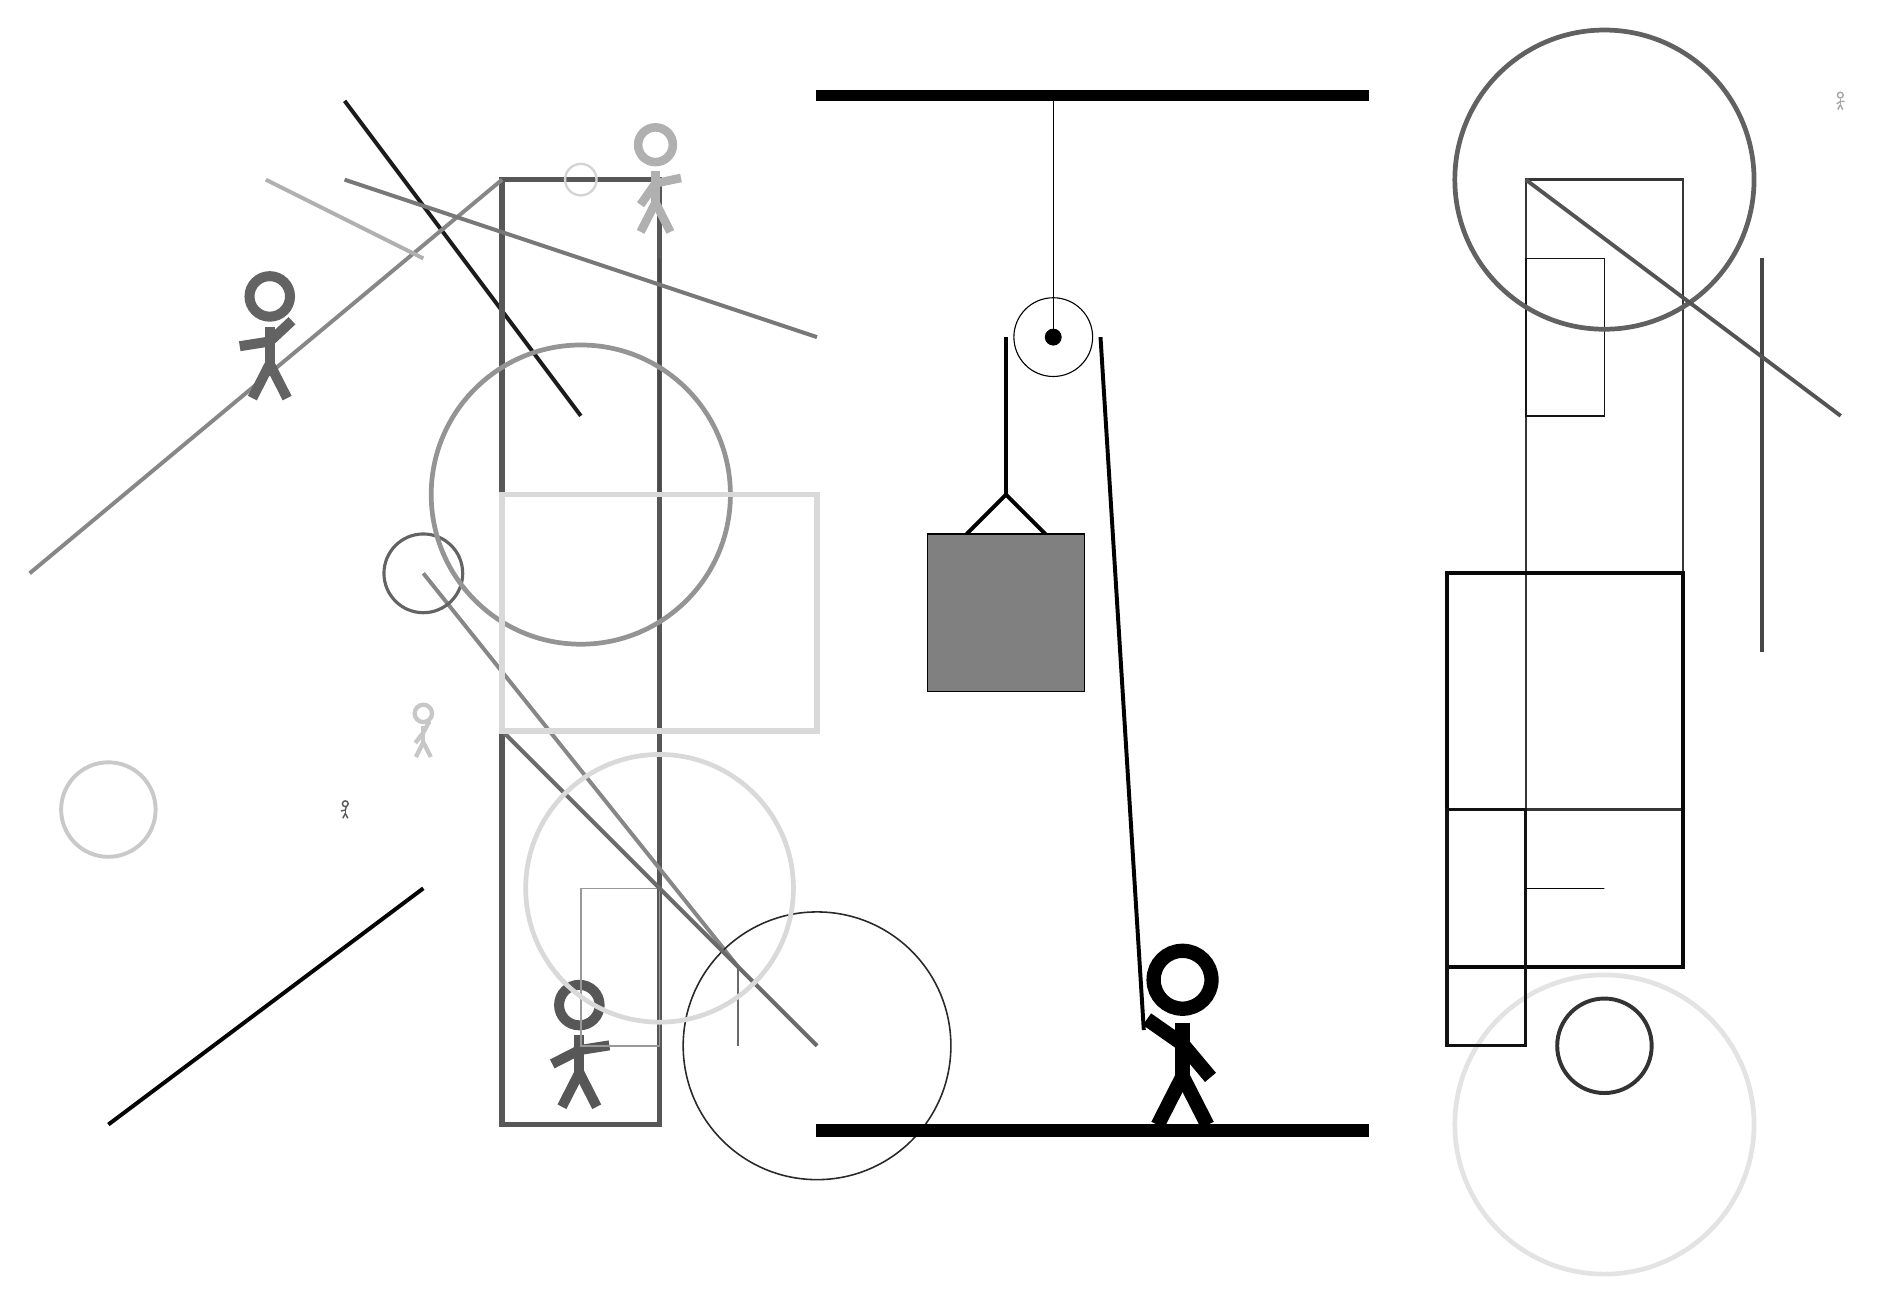
\begin{tikzpicture}
		%%%%% START %%%%%
		
		\draw[fill=black] (-2, 10) rectangle (5, 10.125);
		
		\draw (1, 7) circle (0.5);
		\draw[fill=black] (1, 7) circle (0.1);
		\draw (1, 10) -- (1, 7);
		
		\draw[line width=0.3mm, color=black!79] (7, 1) rectangle (9, 9);
		
		\draw[line width=0.5mm, color=black!72](10, 3) -- (10, 8);
		\draw[line width=0.5mm, color=black!89](-5, 6) -- (-8, 10);
		\draw[line width=0.7mm, color=black!66] (-4, -3) rectangle (-6, 9);
		
		\node[line width=0.5mm, color=black!31] at (-4, 9) {\Strichmaxerl[6][55][12]};
		\draw[line width=0.5mm, color=black!97] (6, -1) rectangle (9, 4);
		\node[line width=0.3mm, color=black!65] at (-8, 1) {\Strichmaxerl[1][9][75]};
		
		\node[line width=0.5mm, color=black!66] at (-5, -2) {\Strichmaxerl[7][27][9]};
		\draw[line width=0.4mm, color=black!71] (-4, 8) rectangle (-4, 5);
		
		\draw[line width=0.2mm, color=black!40] (-4, -2) rectangle (-5, 0);
		
		\draw [line width=0.6mm, color=black!11](8, -3) circle (1.9);
		\node[line width=0.4mm, color=black!22] at (-7, 2) {\Strichmaxerl[3][52][62]};
		\draw[line width=0.4mm, color=black!93] (7, 1) rectangle (6, -2);
		
		\draw[line width=0.5mm, color=black!47](-3, -1) -- (-7, 4);
		\draw [line width=0.5mm, color=black!21](-11, 1) circle (0.6);
		\draw[line width=0.5mm, color=black!47](-6, 9) -- (-12, 4);
		
		\node[line width=0.3mm, color=black!61] at (-9, 7) {\Strichmaxerl[7][9][43]};
		\draw [line width=0.4mm, color=black!61](-7, 4) circle (0.5);
		\draw [line width=0.6mm, color=black!42](-5, 5) circle (1.9);
		\draw[line width=0.5mm, color=black!31](-7, 8) -- (-9, 9);
		\draw [line width=0.2mm, color=black!84](-2, -2) circle (1.7);
		
		\draw[line width=0.5mm, color=black!58](-2, -2) -- (-6, 2);
		
		\draw[line width=0.5mm, color=black!99](-7, 0) -- (-11, -3);
		\draw [line width=0.5mm, color=black!80](8, -2) circle (0.6);
		\draw[line width=0.5mm, color=black!53](-2, 7) -- (-8, 9);
		\draw[line width=0.2mm, color=black!92] (7, 6) rectangle (8, 8);
		\draw[line width=0.2mm, color=black!97] (7, 0) rectangle (8, 0);
		\draw [line width=0.6mm, color=black!62](8, 9) circle (1.9);
		
		\draw[line width=0.5mm, color=black!67](7, 9) -- (11, 6);
		\node[line width=0.3mm, color=black!34] at (11, 10) {\Strichmaxerl[1][33][2]};
		\draw[line width=0.3mm, color=black!58] (-3, -1) rectangle (-3, -2);
		
		\draw [line width=0.6mm, color=black!15](-4, 0) circle (1.7);
		\draw[line width=0.7mm, color=black!15] (-2, 5) rectangle (-6, 2);
		
		\draw [line width=0.3mm, color=black!17](-5, 9) circle (0.2);
		
		\draw[line width=0.5mm] (-0.1, 4.5) -- (0.4, 5.0) -- (0.9, 4.5);
		\draw[fill=black!50] (-0.6, 4.5) rectangle (1.4, 2.5);
		
		\draw[line width=0.5mm] (0.4, 7) -- (0.4, 5.0);
		\centerarc[line width=0.5mm](1, 7)(0:180:0.6);
		\draw[line width=0.5mm](1.6, 7) -- (2.15, -1.8);
		
		\node at (2.6, -1.9) {\Strichmaxerl[10][-35][-50]};
		
		\draw[fill=black] (-2, -3) rectangle (5, -3.15);
		
		%%%%% END %%%%%
	\end{tikzpicture}
\end{document}